%! suppress = UnresolvedReference
\documentclass[11pt,a4paper]{article}

% for Chinese
\usepackage{fontspec}
\newfontfamily\chinesefont{Heiti TC} % Font for Chinese

% useful packages
\usepackage{amsmath}
\usepackage{textcomp}
\usepackage{multirow}
\usepackage{url}
\usepackage{mathtools}
\usepackage{enumitem}
\setlist[itemize]{itemsep=0pt, topsep=0pt}
\setlist[enumerate]{itemsep=0pt, topsep=0pt}
\usepackage{authblk}
\usepackage{algorithm}
\usepackage{hyperref}
\usepackage[capitalize]{cleveref}
\usepackage{amsfonts}
\usepackage[backend=biber,style=alphabetic]{biblatex}
\usepackage{csquotes}
\addbibresource{references.bib}



% basic settings
\renewcommand{\baselinestretch}{1.25}
\parskip=5pt
\parindent=20pt
\footnotesep=5mm

\title{Optimizing Consensus Building in vTaiwan Using Integer Programming \\
\large Operations Research, Spring 2025 (113-2) \\ Group M Final Project Proposal}

\author{b09607059 {\chinesefont 蔡宜芳}, b12705014 {\chinesefont 陳泊華},
    b12705027 {\chinesefont 徐郁翔}, T13H06312 Philip, T13H06303 Kuehnel Paul}
\affil{Department of Information Management, National Taiwan University}

\begin{document}
\maketitle


\begin{abstract}

\centering
This paper formulates and solves an optimization problem for assigning participants
in the vTaiwan process to deliberative groups.
We balance intra-group diversity, stakeholder fairness, and engagement,
while adhering to theoretically grounded group size constraints.

\end{abstract}

\newpage

\section{Introduction}\label{sec:intro}
The \href{https://vtaiwan.tw}{vTaiwan} platform is a widely studied model of digital democracy,
combining online participation with structured, in-person deliberation to inform public policy in Taiwan.
Despite its success, vTaiwan faces persistent challenges such as \textit{group polarization},
\textit{unbalanced participation}, and \textit{inefficient consensus formation}.

For example, in the deliberation on
\href{https://blog.pol.is/uber-responds-to-vtaiwans-coherent-blended-volition-3e9b75102b9b}{Uber's legality},
tech-savvy users and gig economy advocates dominated the discussion,
marginalizing traditional taxi drivers.
In the alcohol sales debate, participation skewed toward industry and libertarian voices,
with little input from public health stakeholders~\parencite{tiku2018taiwan}.
These cases illustrate how self-selection and opinion clustering can lead to echo chambers
and suppress diverse perspectives.

Currently, vTaiwan's deliberation phase uses \href{https://pol.is/home}{Pol.is},
which analyzes voting patterns to cluster participants by opinion similarity
and generate consensus statements that reflect shared views across diverse groups.
While this helps identify areas of agreement,
Pol.is does \textit{not} assign participants into discussion groups for deliberation.
In practice, this means that each group may still contain participants with opposing views
or from conflicting stakeholder backgrounds.

To improve deliberative quality and ensure balanced representation,
we propose moving beyond passive opinion clustering
toward structured group formation methods that explicitly optimize for diversity, fairness, and engagement.

\subsubsection*{Context: Deliberation and Group Design}

Research in deliberative democracy shows that group composition
significantly affects discussion quality~\parencite{fay2000group}.
Small, diverse groups reduce risks of domination
and foster more robust consensus formation~\parencite{anagnostopoulos2012groupformation}.
Odd-numbered group sizes between 5 and 13 are especially effective,
balancing inclusiveness with coordination,
and avoiding decision deadlocks~\parencite{fishkin2009deliberative, menon2011oddgroups}.

Ensuring fairness requires deliberate attention to stakeholder affiliation, opinion diversity,
and participant engagement.
Unstructured group formation can reproduce existing inequalities
or concentrate influence among dominant voices.

\subsubsection*{Project Overview}

This project introduces an optimization-based approach
to deliberative group formation for platforms like vTaiwan.
Instead of relying on emergent clustering,
we model group assignment as a constrained Integer Programming (IP) problem.
Each participant is represented by a feature vector derived from engagement metrics
(comment count, voting behavior, sentiment, stakeholder tags).
Our objective is to generate groups that:
\begin{enumerate}
  \item Maximize intra-group diversity;
  \item Prevent any stakeholder group from dominating too many groups;
  \item Balance engagement levels (and optionally sentiment) across groups.
\end{enumerate}
Group sizes are constrained to odd numbers from $\{5,7,9,11,13,15\}$.
We formulate a formal IP model to encode these goals and constraints,
and explore its linear relaxation to assess tractability and approximation quality.


\section{Background and Related Work}\label{sec:background}
%\subsubsection*{The Role of Group Deliberation in Digital Democracy}
Digital democracy platforms like vTaiwan seek to turn diverse public input into actionable consensus.
While online engagement collects wide-ranging views, small face-to-face deliberations help participants
exchange reasons, clarify misunderstandings, and negotiate trade-offs in real time—enhancing empathy,
reducing polarization, and strengthening trust.
These interpersonal processes are essential complements to algorithmic aggregation.

\subsubsection*{Empirical Findings on Deliberative Group Sizes}\label{subsec:group_sizes}

Studies show a trade-off between inclusiveness and interaction quality.
Small groups (3–5 members) promote balanced, interactive dialogue~\parencite{fay2000group},
while mid-sized groups (8–15) offer more diversity with manageable
coordination~\parencite{involve_citizensjury, fishkin2009deliberative}.
Very large groups often suffer from monologues and disengagement.
Odd-numbered group sizes reduce decision deadlocks and polarization~\parencite{menon2011oddgroups},
making sizes like 5, 7, or 9 both empirically and procedurally robust.

Assuming only about 10\% of the 1921 participants opt into in-person deliberation,
we expect roughly 15–30 groups of 3–13 participants each.

\subsubsection*{Challenges in Group Formation}

Naive clustering approaches (e.g., k-means) often ignore fairness and deliberative quality,
leading to echo chambers or imbalanced groups.
Such methods offer limited control over group sizes or stakeholder representation.

\subsubsection*{Optimization Approaches to Group Design}

Integer Programming (IP) and related techniques have been used for fair team formation and clustering
with explicit constraints~\parencite{anagnostopoulos2012groupformation, celis2018fair}.
Though computationally intensive, these approaches are tractable at vTaiwan’s scale and offer
fine-grained control over group diversity, size, and fairness.


\section{Problem Formulation}\label{sec:problem_formulation}
Let:
\begin{itemize}
    \item $P = \{1, 2, \dots, n\}$: Set of participants.
    \item $G = \{1, 2, \dots, m\}$: Set of groups.
    \item $S = \{1, 2, \dots, r\}$: Set of stakeholder groups.
    \item $s(i) \in S$: Stakeholder group membership of participant $i$.
    \item $D(i,k)$: Diversity score between participants $i$ and $k$.\\(e.g., ideological distance.)
    \item $E(i)$: Engagement score of participant $i$.\\(e.g., number of distinct issues voted on.)
    \item $x_{ij} \in \{0,1\}$: Indicating whether participant $i$ is assigned to group $j$.
    \item $y_{jl} \in \{0,1\}$: Indicating whether group $j$ has size $l \in \{5,7,9,11,13,15\}$.
    \item $z_j \geq 0$: Auxiliary variable representing the absolute deviation of group $j$'s engagement from the target $\bar{E}$.
    \item $d_j \in \{0,1\}$: Binary variable indicating whether group $j$ is dominated by any stakeholder group.
\end{itemize}

Define group size as:
\[
s_j \coloneqq \sum_{i \in P} x_{ij}
\]

\subsection*{Objective Function}

We formulate a composite objective that balances intra-group diversity and engagement fairness:

\[
\max \left[
\lambda_1 \cdot \overbrace{
\sum_{j \in G} \sum_{\substack{i \in P, k \in P \\ i < k}} D(i,k)\,x_{ij} x_{kj}
  }^{\text{(A) Intra-group Diversity}}
\hspace{0.2cm} - \hspace{0.2cm} \lambda_2 \cdot \hspace{-1.3cm} \overbrace{
\sum_{j \in G} z_j
}^{\text{(B) Engagement Imbalance}}
\right]
\]

\noindent
\textbf{(A) Intra-group Diversity:}\\[3pt]
Rewards group compositions that contain participants with a range of differing perspectives.
Diversity scores \(D(i,k)\) are precomputed based on ideological dissimilarity or voting disagreement.
\\
\textbf{(B) Engagement Imbalance:}\\[3pt]
Penalizes uneven distribution of participant engagement across groups by minimizing the total absolute deviation
from a target engagement level \(\bar{E}\).
\\
\textbf{Hyperparameter Tuning:}\\[3pt]
To interpret and calibrate \(\lambda_1\) and \(\lambda_2\), we analyze the individual objective components (A)
and (B) independently.
Each term is normalized (e.g., via max-min or standard deviation scaling)
to ensure their relative importance is interpretable and tunable.

\subsection*{Constraints}
\textbf{(1) Unique Assignment}\\[3pt]
Each participant must be assigned to exactly one group:
\[
\sum_{j \in G} x_{ij} = 1 \quad \forall i \in P
\]
\\
\textbf{(2) Discrete Group Sizes}\\[3pt]
Each group must have a size from the set \(\{5,7,9,11,13,15\}\).
We enforce this using:
\begin{gather*}
    s_j = \sum_{i \in P} x_{ij} \quad \forall j \in G\\
    \sum_{l \in \{5,7,9,11,13,15\}} y_{jl} = 1 \quad \forall j \in G\\
    s_j = \sum_{l \in \{5,7,9,11,13,15\}} l \cdot y_{jl} \quad \forall j \in G
\end{gather*}
\textbf{(3) Diversity Threshold}\\[3pt]
To avoid excessive internal conflict, each group's diversity must not exceed a maximum threshold:
\[
\sum_{i < k} D(i,k)\,x_{ij} x_{kj} \leq \delta \quad \forall j \in G
\]
\textbf{(4) Minimum Engagement per Group}\\[3pt]
Each group must contain a minimum total engagement score:
\[
\sum_{i \in P} E(i)\,x_{ij} \geq \eta \quad \forall j \in G
\]
\textbf{(5) Engagement Deviation Linearization}\\[3pt]
We define the absolute deviation of each group's engagement from the target \(\bar{E}\) using auxiliary variables:
\begin{gather*}
    \sum_{i \in P} E(i)\,x_{ij} - \bar{E} \leq z_j \quad \forall j \in G\\
    \bar{E} - \sum_{i \in P} E(i)\,x_{ij} \leq z_j \quad \forall j \in G\\
\end{gather*}
\textbf{(6) Stakeholder Dominance Control}\\[3pt]
To prevent any stakeholder group from dominating too many groups, we restrict the number of groups
in which more than a threshold fraction \(\alpha\) of members come from the same stakeholder group.

Let \(I_\sigma = \{i \in P \mid s(i) = \sigma\}\) denote the set of participants from stakeholder group \(\sigma \in S\).
Then:
\begin{gather*}
    \sum_{i \in I_\sigma} x_{ij} \leq \alpha \cdot s_j + M \cdot d_j \quad \forall j \in G,\ \forall \sigma \in* S\\
    \sum_{j \in G} d_j \leq \gamma\\
\end{gather*}
% \vspace{-0.5cm}
Where:
\begin{itemize}
    \item \(\alpha \in (0.5, 1)\): Dominance threshold (e.g., \(\alpha = 0.5\) for majority control)
    \item \(d_j \in \{0,1\}\): Indicator whether group \(j\) is dominated
    \item \(M\): Large constant (e.g., \(M = 13\)) to linearize the conditional logic
    \item \(\gamma\): Maximum of allowed dominated groups (e.g., \(\gamma = \lceil 0.05 \cdot |G| \rceil\))
\end{itemize}
\noindent
\subsection*{Constraint Threshold Calibration}
\textbf{Diversity Threshold \(\delta\):}\\[3pt]
Empirically selected from the distribution of intra-group diversity scores in observed or simulated groupings.
Typical values include the 75th or 90th percentile of feasible groupings.
\noindent
\textbf{Engagement Threshold \(\eta\):}\\[3pt]
Derived from desired minimum engagement per group.
For example, if three highly active participants per group are desired,
set \(\eta = 3 \cdot \bar{E}_{\text{individual}}\).

\subsection*{Optional LP Relaxation}

To improve scalability, we relax the binary and discrete constraints as follows:
\begin{itemize}
    \item Assignment variables: \quad $x_{ij} \in \{0,1\}$ is relaxed to $x_{ij} \in [0,1]$.
    \item Group sizes: \quad $s_j \in \{5,7,9,11,13,15\}$ is relaxed to $5 \leq s_j \leq 15$.
    \item Dominance indicators: \quad $d_j \in \{0,1\}$ can be relaxed to $d_j \in [0,1]$ in LP versions with appropriate rounding afterward.
\end{itemize}
We may apply rounding and post-processing to recover feasible integral solutions from the relaxed model.


\section{Summary and Design Justifications}\label{sec:design}
\subsubsection*{Summary and Justification of Design Choices}

This model balances ideological diversity and active participation in forming deliberative groups.
Constraints enforce odd-sized group sizes, regulate stakeholder diversity, and ensure fairness in participant engagement.
By integrating these factors into a single optimization framework, the model supports the formation of high-quality,
balanced groups well-suited for productive democratic deliberation.
Capping stakeholder dominance across groups safeguards against agenda capture
and supports procedural fairness in group composition.

\subsubsection*{Odd-Sized Groups}
Group sizes are restricted to odd values in the set $\{5,7,9,11,13\}$ to avoid deadlocks in binary decisions
and promote more inclusive, decisive deliberation~\parencite{menon2011oddgroups}.
See also Section~\ref{subsec:group_sizes} for empirical justification.

\subsubsection*{Promoting Diversity}
The objective function rewards heterogeneous group compositions based on precomputed dissimilarity scores $D(i,k)$
between participants. These scores can reflect ideological differences, issue preferences, or affective sentiment.

\subsubsection*{Fair Stakeholder Representation}
To avoid group capture by dominant interests, constraints limit the number of groups
in which any stakeholder identity forms a majority. This is controlled via a per-group dominance threshold $\alpha$
and a global cap $\gamma$ on the number of dominated groups.

\subsubsection*{Balanced Engagement}
Participants are scored using engagement metrics $E(i)$, reflecting prior activity (e.g., issues voted on, comments rated).
The model distributes engagement levels evenly across groups by minimizing deviations from a global target $\bar{E}$.
This helps prevent overconcentration of highly active users and encourages balanced group dynamics.




\section{Solution Approach}\label{sec:solution}
\subsection*{Model Implementation}
\subsection*{Solvers and Computational Tools}
\subsection*{Scalability and Complexity Considerations}

\section{Experiments and Results}\label{sec:experiments}
\subsection*{Dataset Description}
\subsection*{Baseline Comparisons}
\subsection*{Performance Metrics}
\subsection*{Analysis and Discussion}

\section{Performance Analysis}\label{sec:performance}
\section{Analysis and Discussion}

\subsection{Experimental Design}

To comprehensively evaluate the performance of different methods under varying problem scales and constraints, we construct nine distinct scenarios, each defined by a unique combination of total participant number $n \in \{50, 300, 1000\}$ and maximum group size $s_{\max} \in \{15, 30, 50\}$. For each scenario, we generate three randomized instances using different seeds ($\text{seed} \in \{0, 1, 2\}$), resulting in a total of 27 experiments.

In each instance, we synthetically generate two key data matrices:
\begin{itemize}
    \item \textbf{Diversity Matrix} $D \in \mathbb{R}^{n \times n}$: Created using a clustered distribution to simulate affinity-based or subgroup-specific dissimilarities among participants.
    \item \textbf{Engagement Vector} $E \in \mathbb{R}^n$: Generated from a normal distribution to simulate varying levels of individual engagement or willingness to contribute.
\end{itemize}

Each method is evaluated based on its assignment of individuals into groups, subject to group size constraints (no more than $s_{\max}$ per group). The objective is to maximize overall diversity within groups while maintaining balanced engagement across them. The weighting parameters for the objective function are set to $\lambda_1 = 1.0$ and $\lambda_2 = 0.0001$.

The methods compared include:
\begin{itemize}
    \item \textbf{Naive Baseline}: Random modulo-based assignment.
    \item \textbf{Heuristic Composite (Random Improvement iteration)}: An iterative method combining subgradient optimization and local search, with a maximum of 2000 iterations.
    \item \textbf{Integer Programming (IP) with Lagrangian Relaxation}: Solved via Gurobi, using binary variables and a decomposition-based reformulation. The solver runs for up to 600 iterations.
    \item \textbf{Linear Programming (LP) Relaxation with Lagrangian Relaxation}: Similar to IP, but allows fractional group assignment variables in $[0, 1]$, also capped at 600 iterations.
\end{itemize}

For each method and instance, we record the following metrics:
\begin{itemize}
    \item \textbf{Optimality Gap (\%)}: Relative gap to the IP+Lagrangian solution (baseline).
    \item \textbf{Execution Time (s)}: Measured using wall-clock time via \texttt{time.perf\_counter()}.
\end{itemize}

All results are aggregated by scenario and reported as averages across three seeds. The IP+Lagrangian method serves as the reference for computing optimality gaps.


\subsection{Motivation for Lagrangian Approach}

Solving the full integer program (IP) to optimality is computationally intensive and becomes intractable for large-scale group deliberation scenarios, especially when the number of participants and grouping constraints increase. In our preliminary tests, even with a powerful solver like Gurobi, solving the exact IP model required hundreds of seconds per instance. To alleviate this, we introduce a Lagrangian-based decomposition approach that retains modeling fidelity while significantly reducing computation time.

Instead of relying on brute-force search or complete enumeration, we reformulate the group assignment problem using Lagrangian relaxation to decouple constraints, enabling more efficient optimization. In practice, we set the maximum number of iterations to \textbf{2000} for the heuristic method, and \textbf{600} for both the IP with Lagrangian relaxation and LP relaxation, ensuring a fair and controlled comparison across methods.

\subsection{Baseline Comparisons}

To evaluate the effectiveness of the proposed Lagrangian Decomposition (LD) method for the group assignment problem, we compare it against the following baselines:

\begin{itemize}
    \item \textbf{Naive Baseline}: Random assignment without any optimization.
    \item \textbf{Heuristic Composite}: A custom-designed heuristic using subgradient methods and local search to iteratively improve solutions as mentioned above.
    \item \textbf{Integer Programming (IP) with Lagrangian Relaxation}: Solved using Gurobi with binary decision variables and Lagrangian reformulation.
    \item \textbf{Linear Programming (LP) Relaxation with Lagrangian Relaxation}: Similar to IP but relaxes binary variables to continuous values in $[0, 1]$.
\end{itemize}

The first two approaches are solver-free and scalable, while the latter two serve as performance upper bounds using commercial optimization software.

\subsection{Performance Metrics}

We use the following metrics to evaluate each method:

\begin{itemize}
    \item \textbf{Optimality Gap (\%)}: Measures how far a method's solution is from the best-known IP value. As this is a maximization problem, the gap is defined as:
    \[
    \text{Gap} = \frac{\text{Optimal Value} - \text{Method Value}}{|\text{Optimal Value}|} \times 100
    \]
    A smaller gap indicates a better solution.
    
    \item \textbf{Standard Deviation (Std)}: Captures the variation in results across repeated trials and reflects robustness.
    
    \item \textbf{Execution Time (seconds)}: Measures the average runtime of each method, important for practical deployment and scalability.
\end{itemize}

All experiments were conducted on the same hardware platform (Apple M-series CPU), and each setting was repeated three times to compute averages and deviations.

\subsection{Optimality Gap}

\textbf{Average Optimality Gap by Scenario} illustrates the average optimality gaps across nine different scenarios, defined by combinations of $(n, s_{\max})$. The IP Lagrangian solution serves as the benchmark baseline (gap = 0\%). 

Among the three heuristics, the \textbf{Random Improvement Iteration Heuristic} consistently outperformed the Naive heuristic. For instance, in the largest instance $(n=1000, s_{\max}=15)$, the CHSF gap was approximately 75.0\%, compared to 887.1\% for the Naive heuristic—a reduction of over 91\%. Even in the smallest case $(n=50, s_{\max}=15)$, Random Improvement Iteration yielded a gap of 16.2\%, still substantially lower than the Naive heuristic's 140.2\%.

The LP Relaxation method achieved near-zero gap in most scenarios (0\% except 0.4\% in the largest instance), affirming its tight bound but at the cost of high computation time, as discussed below.

\begin{figure}[H]
    \centering
    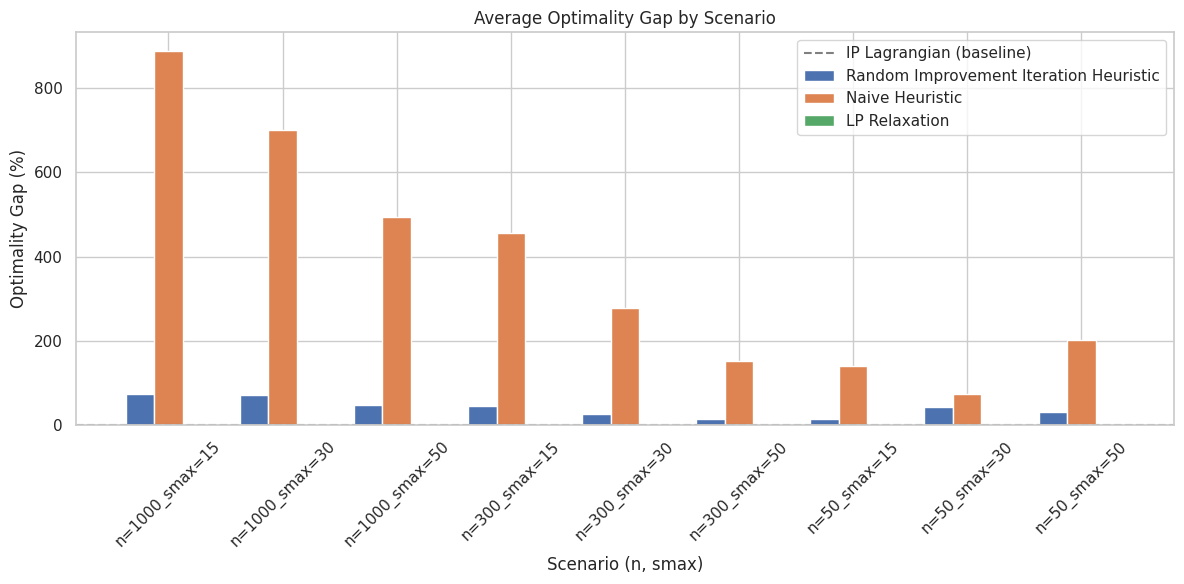
\includegraphics[width=0.8\textwidth]{assets/gap.png}
    \caption{Average Optimality Gap by Scenario}
    \label{fig:your-label}
\end{figure}

\subsection{Computation Time}

\textbf{Figure 2} presents the average computation time on a logarithmic scale. While the Naive heuristic completed in under 0.01 seconds for all scenarios (e.g., 0.007s in $(n=1000, s_{\max}=15)$), Random Improvement Iteration required more time due to its iterative improvement steps—e.g., 1.35s in the same instance. Nevertheless, this is still orders of magnitude faster than LP Relaxation, which took over 413 seconds.

Interestingly, Random Improvement Iteration provided a strong balance between solution quality and computational efficiency. Across all settings, it achieved substantial gap reduction compared to the Naive approach while keeping runtime within practical limits (all under 1.4 seconds). 

\begin{figure}[H]
    \centering
    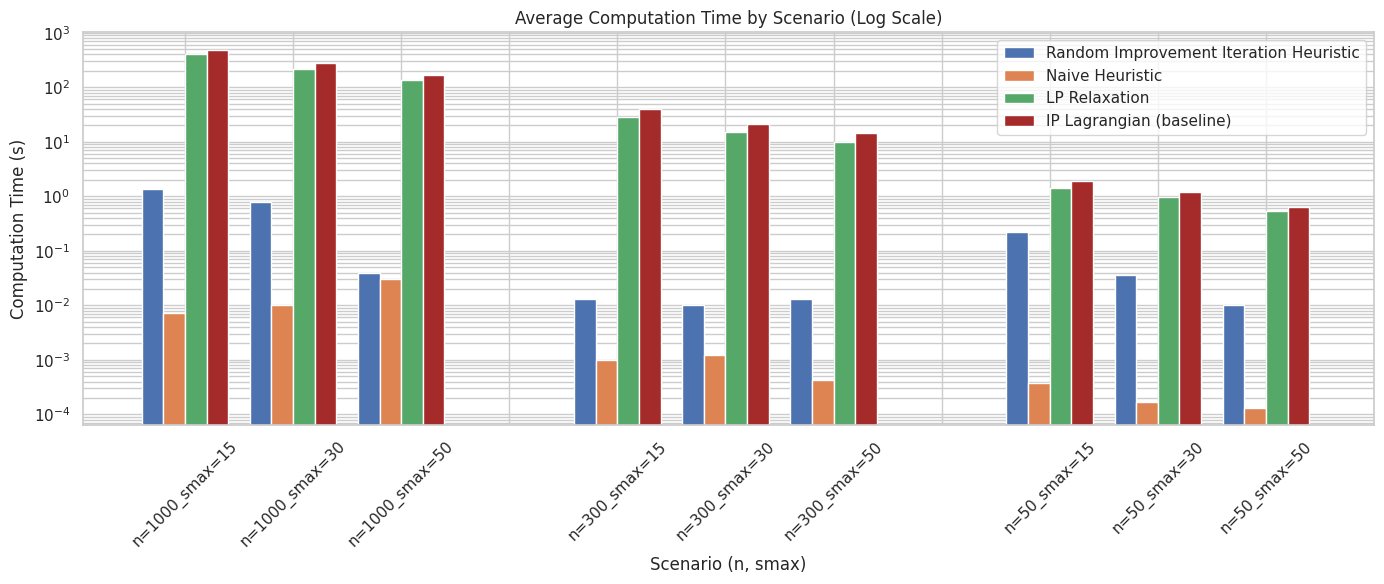
\includegraphics[width=0.8\textwidth]{assets/time.png}
    \caption{Average Computation Time by Scenario (Log Scale)}
    \label{fig:your-label}
\end{figure}

\subsection{Summary}

In summary, the Random Improvement Iteration heuristic demonstrates clear advantages over the Naive baseline in both optimality and scalability. It also provides a viable alternative to LP Relaxation when computational cost is a limiting factor, especially for large-scale instances.

In conclusion, the proposed \textbf{Lagrangian-based heuristic provides a compelling trade-off between solution quality and runtime}. It is especially suitable for large-scale, real-time, or resource-constrained scenarios. Furthermore, the modular structure of the heuristic framework makes it extendable to more general group assignment settings, including multi-objective, multi-stage, or incomplete-information environments.


\section{Conclusion}\label{sec:conclusion}
By formulating the group formation challenge as an integer optimization problem,
we present a flexible and interpretable approach for assigning participants to deliberative groups.
Our model explicitly controls group size, diversity,
and engagement balance—capabilities missing in traditional clustering-based techniques.
The inclusion of a Linear Programming relaxation enables faster solution times for large-scale instances,
making the method practically applicable.
We expect the resulting groups to be more balanced and representative, improving discussion quality
and legitimacy in vTaiwan and similar participatory platforms.

\subsection*{Limitations and Future Work}


\end{document}
